% Created 2021-11-05 Fri 08:15
% Intended LaTeX compiler: pdflatex
\documentclass[presentation,aspectratio=169]{beamer}
\usepackage[utf8]{inputenc}
\usepackage[T1]{fontenc}
\usepackage{graphicx}
\usepackage{grffile}
\usepackage{longtable}
\usepackage{wrapfig}
\usepackage{rotating}
\usepackage[normalem]{ulem}
\usepackage{amsmath}
\usepackage{textcomp}
\usepackage{amssymb}
\usepackage{capt-of}
\usepackage{hyperref}
\usepackage{khpreamble}
\usepackage{amssymb}
\DeclareMathOperator{\shift}{q}
\DeclareMathOperator{\diff}{p}
\usepackage{tcolorbox}
\usetheme{default}
\author{Kjartan Halvorsen}
\date{\today}
\title{From continuous-time to discrete-time systems}
\hypersetup{
 pdfauthor={Kjartan Halvorsen},
 pdftitle={From continuous-time to discrete-time systems},
 pdfkeywords={},
 pdfsubject={},
 pdfcreator={Emacs 26.3 (Org mode 9.4.6)}, 
 pdflang={English}}
\begin{document}

\maketitle

\section{Intro}
\label{sec:orgf5ea9d3}

\begin{frame}[label={sec:org6974285}]{The computerized control system of the Apollo LM}
\begin{columns}
\begin{column}{0.3\columnwidth}
\begin{center}
 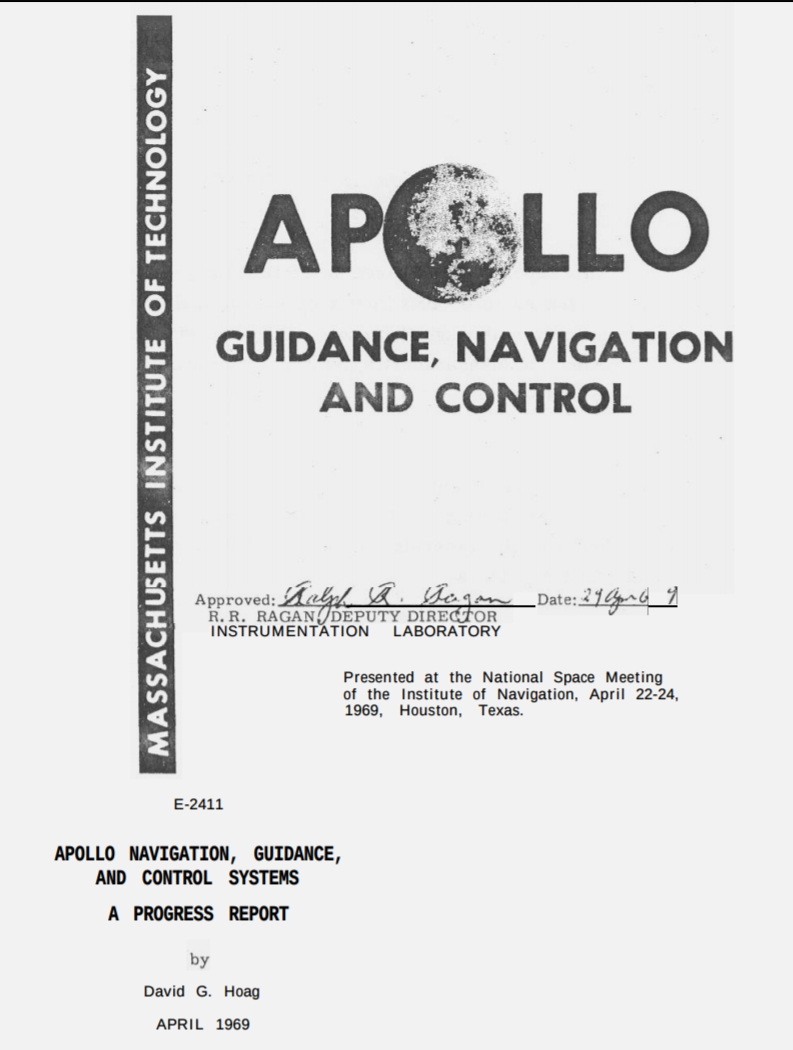
\includegraphics[width=1.0\linewidth]{../../figures/Hoag-report-1.png}
\end{center}
\end{column}
\begin{column}{0.7\columnwidth}
\pause

\begin{center}
 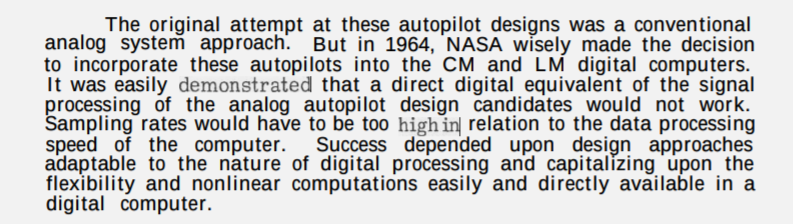
\includegraphics[width=.7\linewidth]{../../figures/Hoag-report-2.png}
\end{center}

\pause

\begin{center}
 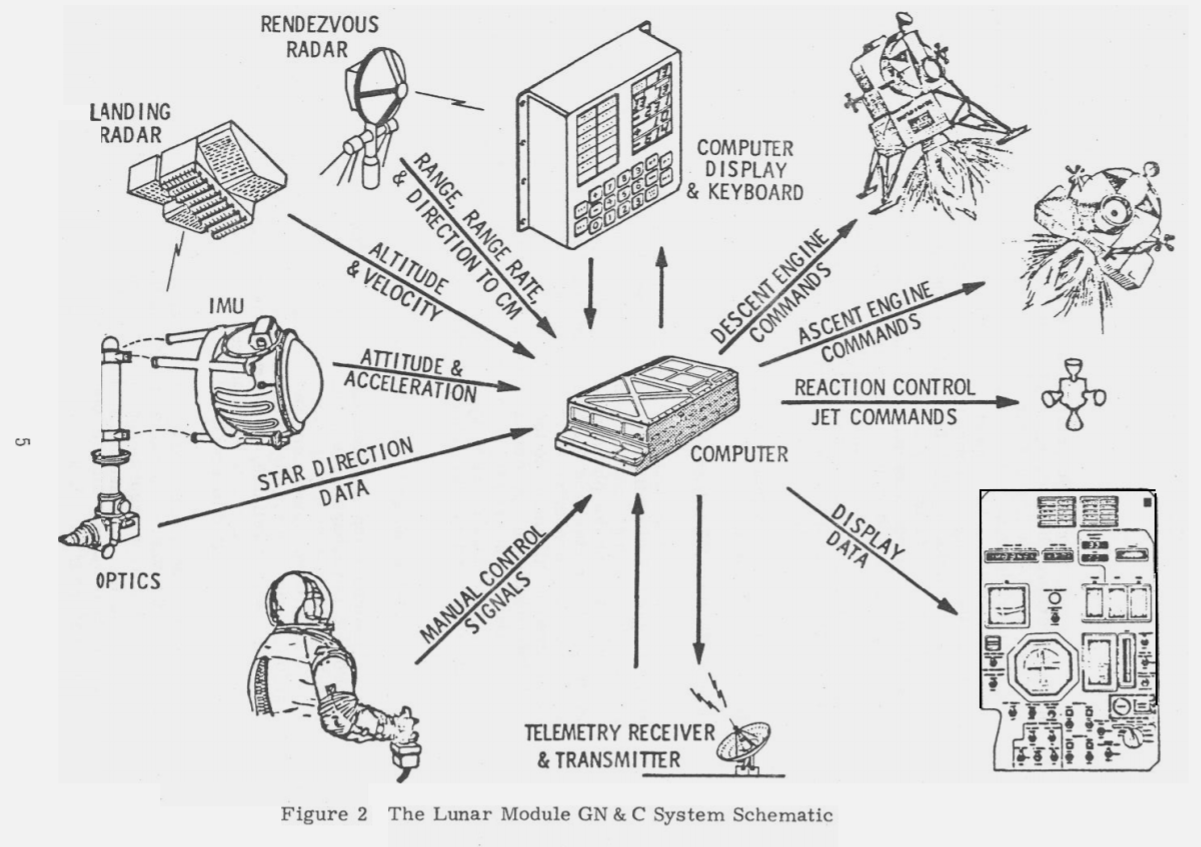
\includegraphics[width=.7\linewidth]{../../figures/Hoag-report-fig2.png}
\end{center}
\end{column}
\end{columns}
\end{frame}

\section{Discrete-time system example}
\label{sec:org7d51b9e}

\section{Zero-order hold, or step-invariant sampling preview}
\label{sec:org17d5437}

\begin{frame}[label={sec:org992311c}]{Discrete-time systems}
\end{frame}


\begin{frame}[label={sec:org8f81bb2}]{The world according to the discrete-time controller}
\small 
\begin{center}
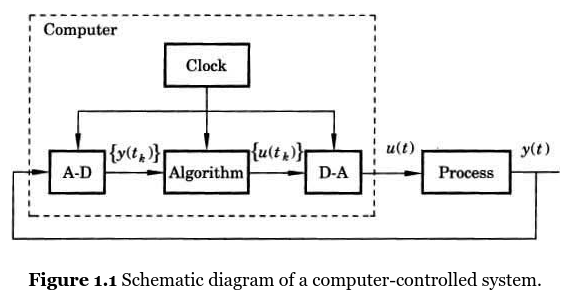
\includegraphics[width=0.6\linewidth]{../../figures/fig1-1-schematic.png}

Source: Åström and Wittenmark "Computer-controlled systems".
\end{center}

\pause

The sampling leading to the \emph{stroboscopic} model can have some peculiar effects: \url{https://youtu.be/yIUZ-qKWnXc}
\end{frame}

\begin{frame}[label={sec:orgb3bc405}]{Discrete-time Linear Shift-Invariant systems}
\begin{center}
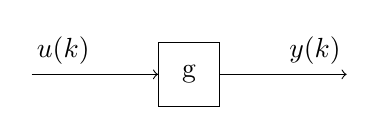
\begin{tikzpicture}[node distance=20mm, anchor=north]
\node[coordinate] (input) {};
\node[rectangle, draw, right of=input, inner sep=3mm] (lti) {g};
\node[coordinate, right of=lti] (output) {};
\draw[->] (input) -- node[near start, above] {$u(k)$}  (lti);
\draw[->] (lti) -- node[near end, above] {$y(k)$} (output);
\end{tikzpicture}
\end{center}

\pause

\begin{block}{General case (non-causal)}
\[ y(k) = g \ast u = \sum_{n=-\infty}^\infty g(n) u(k-n) \]

\pause
\end{block}

\begin{block}{Causal case}
\[ y(k) = g \ast u = \sum_{n=0}^\infty g(n) u(k-n) \]


\(g(k)\) is called the \alert{weighting sequence}.
\end{block}
\end{frame}


\begin{frame}[label={sec:orgd188ba8}]{Discrete-time LSI systems}
\begin{block}{Impulse response}
\[ y(k) = g \ast u = \sum_{n=0}^\infty g(n) u(k-n) \]

If the input signal is a unit discrete impulse

\begin{center}
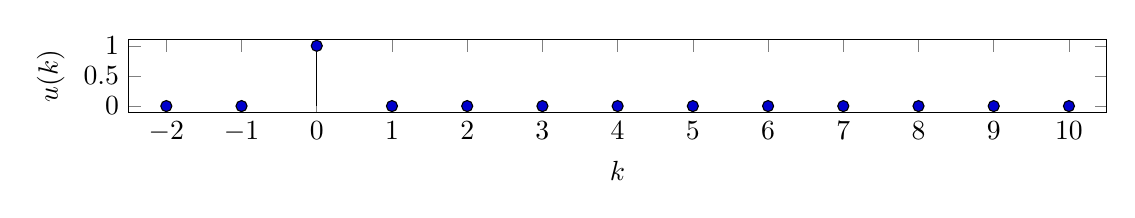
\begin{tikzpicture}
\begin{axis}[
  width=14cm,
  height=2.5cm,
  xlabel={$k$},
  ylabel={$u(k)$},
  xmin=-2.5,
  xmax=10.5,
]

\addplot+[black, ycomb, domain=-2:10, samples=13,variable=k] { (k==0)}; 

\end{axis}
\end{tikzpicture}
\end{center}


\pause

\[ y(k) = \sum_{n=0}^\infty g(n) \delta(k-n) = g(k) \]

\alert{The weighting sequence is equal to the impulse response of the system.}
\end{block}
\end{frame}

\begin{frame}[label={sec:org04c3c97}]{The response of a discrete LSI system is a weighted sum of the current and previous values of the input}
\small

\[ y(k) = g \ast u = \sum_{n=0}^\infty g(n) u(k-n) \]


\alert{Activity} What is the response of a system to the input signal \(u(k)\) if its impulse response (weighting sequence) is the one below, \(g(k) = \delta(k-4)\) ?

\begin{center}
\begin{tikzpicture}
\small
\begin{axis}[
  width=14cm,
  height=3.5cm,
  xlabel={$k$},
  ylabel={$g(k)$},
  xmin=-0.5,
  xmax=10.5,
  ytick = {0, 1},
]

\addplot+[black, ycomb, domain=-2:10, samples=13,variable=k] { (k==4)}; 

\end{axis}
\end{tikzpicture}
\end{center}

\[y(k) = \]
\end{frame}
\section{The z-transform}
\label{sec:org107fcff}
\begin{frame}[label={sec:org0ea6969}]{The z-transform}
\end{frame}

\begin{frame}[label={sec:orgc9bf043}]{The impulse modulation model of sampling}
The \alert{impulse train}, a.k.a the \alert{Dirac comb}:
\(m(t) = \sum_{k=-\infty}^{\infty} \delta(t-kh)\)\hspace*{10mm}
\pause
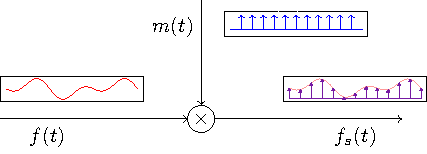
\includegraphics[width=0.4\linewidth]{../../figures/modulation-model-blocks}

\pause

\[f_s(t) = f(t)m(t) = f(t) \sum_{k=-\infty}^{\infty} \delta(t-kh) = \sum_{k=-\infty}^{\infty} f(t)\delta(t-kh) = \sum_{k=-\infty}^{\infty} f(kh) \delta(t-kh) \]


\begin{center}
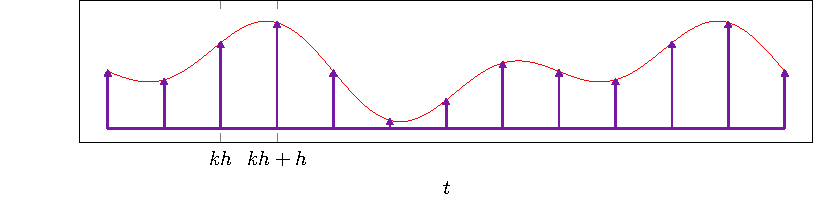
\includegraphics[width=0.8\linewidth]{../../figures/modulation-model-timeseries}
\end{center}
\end{frame}


\begin{frame}[label={sec:orgf81efd7}]{The Laplace transform}
\begin{block}{Definition}
\[ F(s) = \laplace{f(t)} = \int_0^\infty f(t) \mathrm{e}^{-st} dt\]
\end{block}
\begin{block}{Inverse transform}
\[ f(t) = \mathcal{L}^{-1}\{F(s)\} = \frac{1}{2\pi i} \int_{\gamma - i\infty}^{\gamma + i\infty} F(s)\mathrm{e}^{st} \, ds \]

Note that in control engineering, the one-sided transform is used.
\end{block}
\end{frame}

\begin{frame}[label={sec:orgf60fe11}]{The z-transform}
\begin{block}{Definition}
\[ F(z) = \ztrf{f(kh)} = \sum_{k=0}^{\infty} f(kh)z^{-k} \]
\end{block}

\begin{block}{Inverse transform}
\[ f(kh) = \frac{1}{2\pi i} \oint_r F(z) z^{k-1} \, dz \]

Note that in control engineering, the one-sided transform is used.
\end{block}
\end{frame}

\begin{frame}[label={sec:orgda2f547}]{The Laplace transform of a sampled signal}
Assume right-sided signal \(f(t)\), meaning it is zero for negative times \(t<0\).
\[f_s(t) = f(t)m(t) = f(t) \sum_{k=0}^{\infty} \delta(t-kh) = \sum_{k=0}^{\infty} f(t)\delta(t-kh) = \sum_{k=0}^{\infty} f(kh) \delta(t-kh) \]

\pause

\begin{align*}
F_s(s) &= \laplace{f_s(t)} = \int_0^\infty \left(\sum_{k=0}^{\infty} f(kh) \delta(t-kh)\right)\mathrm{e}^{-st}\, dt \\
&= \sum_{k=0}^{\infty} \int_0^\infty  f(kh) \delta(t-kh) \mathrm{e}^{-st}\, dt = \sum_{k=0}^{\infty} f(kh) \mathrm{e}^{-skh}\\
&= \sum_{k=0}^{\infty} f(kh) \left(\mathrm{e}^{sh}\right)^{-k}
\end{align*}
\end{frame}

\begin{frame}[label={sec:org5996013}]{The Laplace transform of a sampled signal}
\small

Note:
\begin{align*}
F_s(s) &=  \sum_{k=0}^{\infty} f(kh) \left(\mathrm{e}^{sh}\right)^{-k}\quad \text{Laplace transform}\\
F(z) &= \sum_{k=0}^{\infty} f(kh) z^{-k} \quad \text{z-transform}
\end{align*}

\alert{Activity} How is the Laplace transform of the sampled signal and the z-transform of the corresponding discrete-time sequence related?

\pause

\begin{tcolorbox}
 The z-transform of a sampled signal corresponds to its Laplace transform with the following relationship between the s-plane of the Laplace transform and the z-plane of the z-plane of the z-transform.
\[ z = \mathrm{e}^{sh}\]
\end{tcolorbox}
\end{frame}


\begin{frame}[label={sec:org245ad09}]{One of the most important transform pairs}
\[f(kh) = \alpha^{kh}, \quad \alpha \in \mathbb{C}\]

\pause

\begin{align*}
   F(z) &= \ztrf{f(kh)} = \sum_{k=0}^{\infty} f(kh)z^{-k}
   =  \sum_{k=0}^{\infty} \alpha^{kh}z^{-k} =  \sum_{k=0}^{\infty} \left(\alpha^{h}\right)^kz^{-k}\\
   &=  \sum_{k=0}^{\infty} \left(\frac{\alpha^{h}}{z}\right)^{k}
   =  \frac{1}{1 - \frac{\alpha^h}{z}} = \frac{z}{z-\alpha^{h}}, \quad |\frac{\alpha^h}{z}| < 1
\end{align*}

\pause

\begin{tcolorbox}
\[ \alpha^{kh} \quad  \overset{\mathcal{Z}}{\longleftrightarrow} \quad \frac{z}{z-\alpha^h} \]
\end{tcolorbox}
\end{frame}

\section{Step-invariant sampling}
\label{sec:org3661187}


\begin{frame}[label={sec:org0cb5ac5}]{Step-invariant sampling (a.k.a ZOH sampling)}
\end{frame}

\begin{frame}[label={sec:orgd25ecf2}]{Step-invariant sampling (a.k.a ZOH sampling)}
\begin{center}
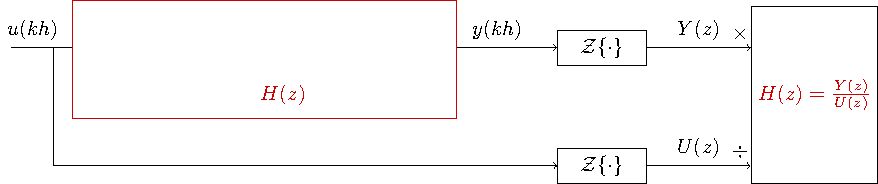
\includegraphics[width=0.9\linewidth]{../../figures/invariant-sampling-white.pdf}
\end{center}

\pause
Step-invariant sampling (zero order hold): \(u(kh) = \begin{cases} 1, & k \ge 0\\0, & k<0 \end{cases}\)
\end{frame}

\begin{frame}[label={sec:orga4100da}]{Step-invariant sampling (a.k.a ZOH sampling)}
The idea is to sample the continuous-time system's response to a step input, in order to obtain a discrete approximation which is \alert{exact} (at the sampling instants) for such an input signal. 

\begin{center}
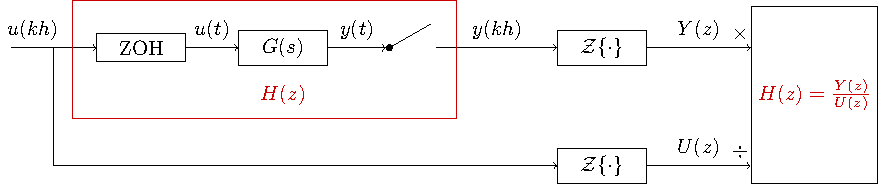
\includegraphics[width=0.9\linewidth]{../../figures/invariant-sampling.pdf}
\end{center}

Step-invariant sampling (zero order hold): \(u(kh) = \begin{cases} 1, & k \ge 0\\0, & k<0 \end{cases}\)
\end{frame}

\begin{frame}[label={sec:org9a2df7c}]{Why is step-invariant sampling a good idea?}
A piecewise constant (stair-case shaped) function can be written as a sum of delayed step-responses!
\begin{center}
  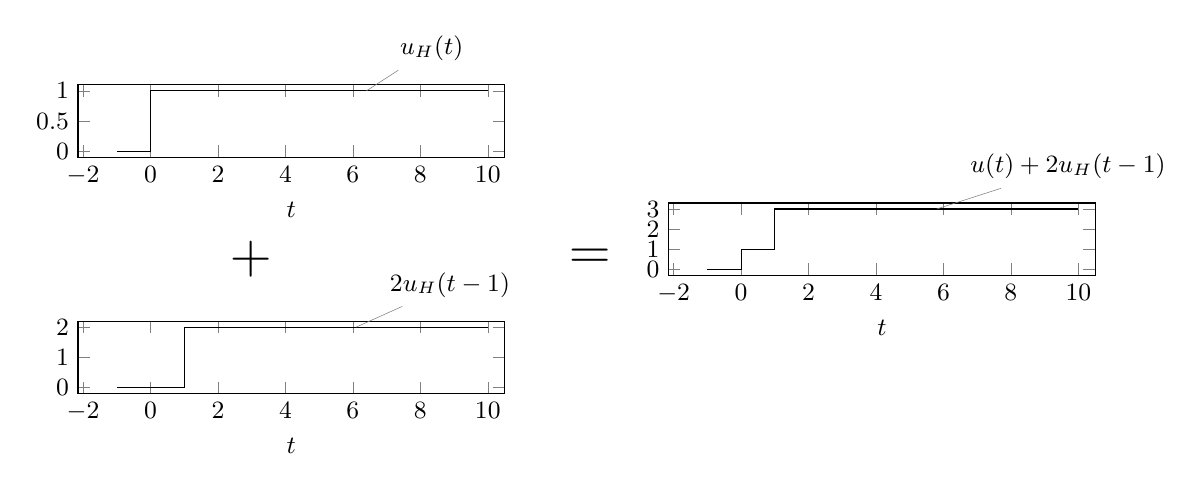
\begin{tikzpicture}
    \small
    \begin{axis}[
      clip = false,
      width=7cm,
      height=2.5cm,
      yshift=1.5cm,
      xlabel={$t$},
      ylabel={},
      xmax=10.5,
      ]
      \addplot+[black, no marks] coordinates {(-1,0) (0,0) (0,1) (10,1) } node[pos=0.7,coordinate, pin=40:$u_H(t)$] {};
    \end{axis}
    \begin{axis}[
      clip=false,
      width=7cm,
      height=2.5cm,
      yshift=-1.5cm,
      xlabel={$t$},
      ylabel={},
      xmax=10.5,
      ]
      \addplot+[black, no marks] coordinates {(-1,0) (1,0) (1,2) (10,2) } node[pos=0.7,coordinate, pin=40:$2u_H(t-1)$] {};;
    \end{axis}
    \begin{axis}[
      clip=false,
      width=7cm,
      height=2.5cm,
      xshift=7.5cm,
      xlabel={$t$},
      ylabel={},
      xmax=10.5,
      ]
      \addplot+[black, no marks] coordinates {(-1,0) (0,0) (0,1) (1,1) (1,3) (10,3) }  node[pos=0.7,coordinate, pin=40:$u(t) + 2u_H(t-1)$] {};;
    \end{axis}

    \node at (2.2,0.2) {\huge  +};
    \node at (6.5,0.2) {\huge  =};

  \end{tikzpicture}
\end{center}
\end{frame}


\section{Zero-order hold sampling procedure}
\label{sec:org7b5acae}
\begin{frame}[label={sec:orgf361638}]{Step-invariant sampling, or zero-order-hold sampling}
Let the input to the continuous-time system be a unit step \(u(t)=u_H(t),\) which has Laplace transform \(U(s)=\frac{1}{s}.\) In the Laplace-domain we get
\[Y(s) = G(s)\frac{1}{s}\]
\begin{enumerate}
\item Obtain the time-response by inverse Laplace: \(y(t)=\laplaceinv{Y(s)}\)
\item Sample the time-response to obtain the sequence \(y(kh)\) and apply  the z-transform to obtain \(Y(z) = \ztrf{y(kh)}\)
\item Calculate the pulse-transfer function by dividing with the z-transform of the input signal \(U(z) = \frac{z}{z-1}.\) \[H(z) = \frac{Y(z)}{U(z)} = \frac{z-1}{z}Y(z) \]
\end{enumerate}
\end{frame}

\section{Zero-order hold sampling example}
\label{sec:org52f7c74}
\begin{frame}[label={sec:org5f312bc}]{Example: First-order system}
\small

\[ G(s) = \frac{1}{\tau s + 1}. \]

\pause
\begin{enumerate}
\item Step response: \(y(t) = \big(1 - \mathrm{e}^{-\frac{t}{\tau}}\big)u_H(t)\)
\end{enumerate}
\pause
\begin{enumerate}
\setcounter{enumi}{1}
\item Sampling and applying the z-transform:
\[ y(kh) = \big(1 - \mathrm{e}^{-\frac{kh}{\tau}}\big)u_H(kh) = u_H(kh) - \big(\mathrm{e}^{-\frac{h}{\tau}}\big)^k u_H(kh) \]
\end{enumerate}
\pause
\begin{align*} Y(z) &= \frac{z}{z-1} - \frac{z}{z-\mathrm{e}^{-\frac{h}{\tau}}} = \frac{z\big(z-\mathrm{e}^{-\frac{h}{\tau}} - (z-1)\big)}{(z-1)(z-\mathrm{e}^{-\frac{h}{\tau}})}
= \frac{z(1-\mathrm{e}^{-\frac{h}{\tau}})}{(z-1)(z-\mathrm{e}^{-\frac{h}{\tau}})}
\end{align*}
\pause
\begin{enumerate}
\setcounter{enumi}{2}
\item Calculate the pulse-transfer function
\[H(z) = \frac{Y(z)}{U(z)} = \frac{z-1}{z} \cdot \frac{z(1-\mathrm{e}^{-\frac{h}{\tau}})}{(z-1)(z-\mathrm{e}^{-\frac{h}{\tau}})} = \frac{1-\mathrm{e}^{-\frac{h}{\tau}}}{z-\mathrm{e}^{-\frac{h}{\tau}}} \]
\end{enumerate}
\end{frame}
\end{document}